%!TEX root = ../dokumentation.tex
\chapter{Planung und Konzeption}
In diesem Kapitel werden die Anforderungen für ein digitales Funkübertragungssystem definiert, welches die Möglichkeit bieten soll beliebige Signale im Bereich der Dezimeterwelle zu analysieren und zu verarbeiten. Das aus dieser Definition resultierende System wird im Verlauf dieses Kapitels geplant und implementiert.\\
Um möglichst viele Dienste im Frequenzbereich der Dezimeterwelle analysieren zu können sollte der Hardwareaufbau, bestehend aus Antenne und digitalem Empfängersystem, folgende Eigenschaften besitzen:
\begin{itemize}
	\item Die Antenne sollte möglichst breitbandig sein. Sie muss mindestens den vorgegeben Bereich zwischen 300 MHz und 3000 MHz abdecken.
	\item Um ein Signal vollständig zu erfassen muss auch das digitale Empfängersystem eine ausreichende Kanalbandbreite aufweisen.
	\item Die Abtastrate des Systems muss gemäß Abschnitt \ref{abtasttheorem} ausreichend hoch sein um das Signal rekonstruieren zu können.
	\item Das System muss mit einem Unix-ähnlichem Betriebssystem oder mit Microsoft Windows bedienbar sein.
	\item Der Dynamikumfang des Systems muss ausreichend groß sein. Dabei ist die untere Grenze erfassbarer Signale das Grundrauschen im System und dessen Umgebung; der Bereich nach oben wird hingegen durch die maximal erfassbare Signalgröße eingeschränkt. %TODO: Irgendo muss der Dynamikumfang erklärt werden. -> Sascha Dynamik eschreibt das Verhältnis zwischen dem größtöglichen zum kleinsmöglichen Pegel bei 40 dB liegt der Unterschied zwischen den Werten bei 1:10 000.
	\item Das System soll unter wirtschaftlichem Gesichtspunkt entworfen werden.
\end{itemize}%TODO: Gibt es noch mehr Anforderungen? Kosten, etc? Datenblatt der Antenne und was aus den Fingern saugen was tolles Schreiben

Die aufgeführten Anforderungen werden bei der Planung des Systems, besonders bei der Auswahl der Hardware, berücksichtigt. Auf den folgenden Seiten wird auf die einzelnen Punkte näher eingegangen. 

Zunächst wird jedoch im Verlauf des Kapitels das Frequenzspektrum der Dezimeterwelle und die rechtlichen Rahmenbedingungen für Dienste in diesem Bereich untersucht, um mögliche Rückschlüsse auf das zu entwerfende System ziehen zu können.


%Die Angabe des Spektrums bietet folgende Vorteile: 

%Das Ergebnis ist in der Regel deutlich präziser. Wenngleich das Oszilloskop wohl das
%wichtigste Messinstrument der Elektrotechnik ist, arbeitet es vergleichsweise ungenau. Es
%liefert dem Anwender einen groben Überblick über die Form des Signals. Bei den ge-
%genwärtig verbreiteten Digitalspeicheroszilloskopen mit 8-bit-Wandler ist die Dynamik
%schon aufgrund der Analog-Digital-Wandlung auf bestenfalls 48dB begrenzt; bei guten
%Spectrum Analyzern erreicht man hingegen 120dB und mehr.


\newpage
\section{Das Frequenzspektrum}
\label{section-frequenzbereiche}
Zur Orientierung im Spektrum elektromagnetischer Wellen haben sich international verschiedene Systeme zur Klassifikation sogenannter Frequenzbänder gebildet. Die \ac{ITU} empfiehlt eine Einteilung des Spektrums von 3 kHz bis 300 GHz in acht Frequenzbereiche, auch Frequenzdekaden genannt. \cite[vgl. ITU-R v.431-8]{itu-431:2015}

\begin{figure}[ht]
	\centering
	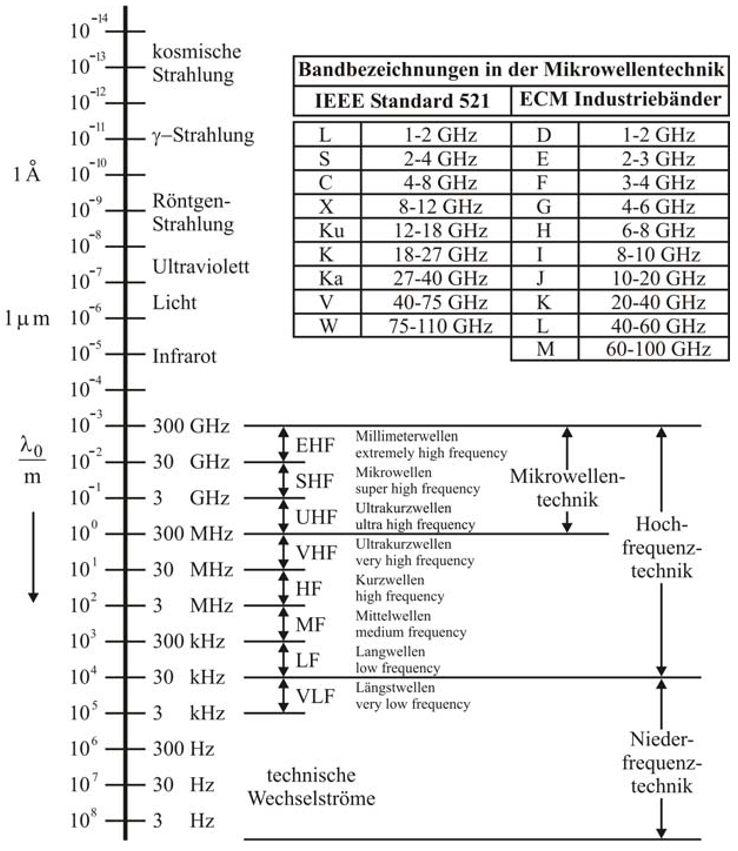
\includegraphics[width=0.75\textwidth]{frequenzbereich.png}
	\caption[Spektrum elektromagnetischer Wellen und gebräuchliche Bandbezeichnungen]{Spektrum elektromagnetischer Wellen und gebräuchliche Bandbezeichnungen. Quelle: \cite[Kark, S. 1]{Kark:2017}} 
	\label{frequenzbereiche}
\end{figure}






\subsection{Rechtliche Grundlagen} %TODO
In Deutschland gilt rechtlich zudem die Aufteilung des Frequenzbereiches von 9 kHz bis 3000 GHz, welche von der Bundesnetzagentur im sogenannten Frequenzplan \cite[Bundesnetzagentur, 2016]{bundesnetzagentur-frequenzplan:2016} gemäß § 54 TKG festgehalten wird.
Dort werden die Frequenzbereiche nach Frequenznutzung (Amateurfunk, Seefunk, WLAN, etc.) eingeteilt und entsprechende Nutzungsbestimmungen spezifiziert:

\begin{figure}[ht]
	\centering
	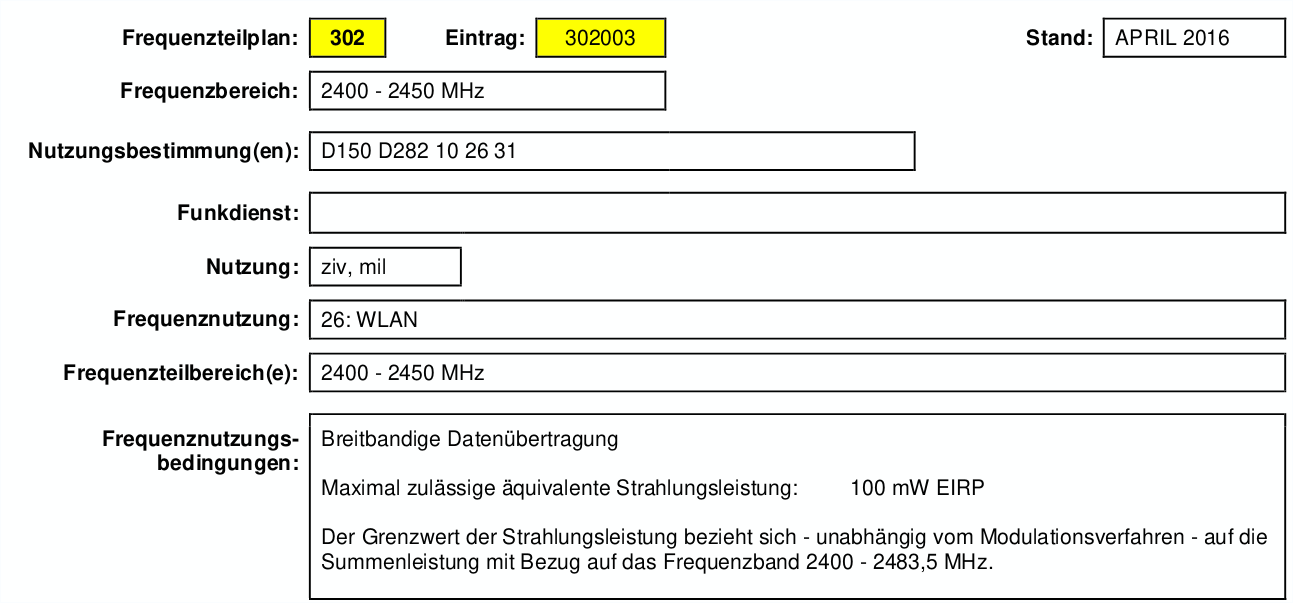
\includegraphics[width=\textwidth]{freqplan-wlan.png}
	\caption[Eintrag: 2,4 GHz WLAN im Frequenzplan]{Eintrag: 2,4 GHz WLAN im Frequenzplan. Quelle: \cite[Bundesnetzagentur, 2016]{bundesnetzagentur-frequenzplan:2016}}
	\label{frequenzplan-wlan}
\end{figure}



\section{Anwendungen im Bereich der Dezimeterwelle}
Das Frequenzband von 300 MHz bis 3 GHz, auch \ac{UHF}-Band genannt, ist ein Frequenzbereich in dem die Wellen eine Länge von zehn Dezimeter bis einem Dezimeter besitzen:
\( \lambda = \frac{c}{f} = \frac{3*10^8 \text{ m/s}}{300 \text{ MHz}} = 1\text{ m}\)
und
\( \frac{3*10^8 \text{ m/s}}{3000 \text{ MHz}} = 0.1\text{ m}\).
Der damit untersuchte Frequenzbereich erstreckt sich von 300 MHz bis 3 GHz. Darunter befinden sich die gängigsten Anwendungen, die im folgenden detaillierte beschrieben werden.

In dem oben genannten Frequenzbereich liegen folgende Anwendungen:

\begin{description}
	\item [Amateurfunkdienste]{}
	\item [Mobile Landfunkdienst] {}
	\item [Wettersatelliten] {}
	\item [DECT] {Digital Enhanced Cordless Telecommunications ist ein internationaler Standard für Telekommunikations mittels Funktechnik häufig bei Schnurlostelefonen. Dieser Standard arbeitet grundsätzlich verbindungsorientiert und ist primär für Telefonie innerhalb von Gebäuden ausgelegt. Deren Reichweite beträgt ca. 30-50 Meter. DECT beschreibt eine reine Zugangstechnologie im Gegensatz zu herkömmlichen Mobilfunksystemen. Der Frequenzbereich bei DECT liegt bei 1880 MHz-1900 MHz.}
	\item [GSM] {}
	\item [GPS] {}
	\item [Bluetooth] {Bluetooth ist ein entwickelter Industriestandard für die Datenübertragung zwischen Geräten über kurze Distanz}
	\item [WLAN] {}
\end{description}

\section{Spektralanalyse der Dezimeterwelle}
\begin{figure}[ht]
	\centering
	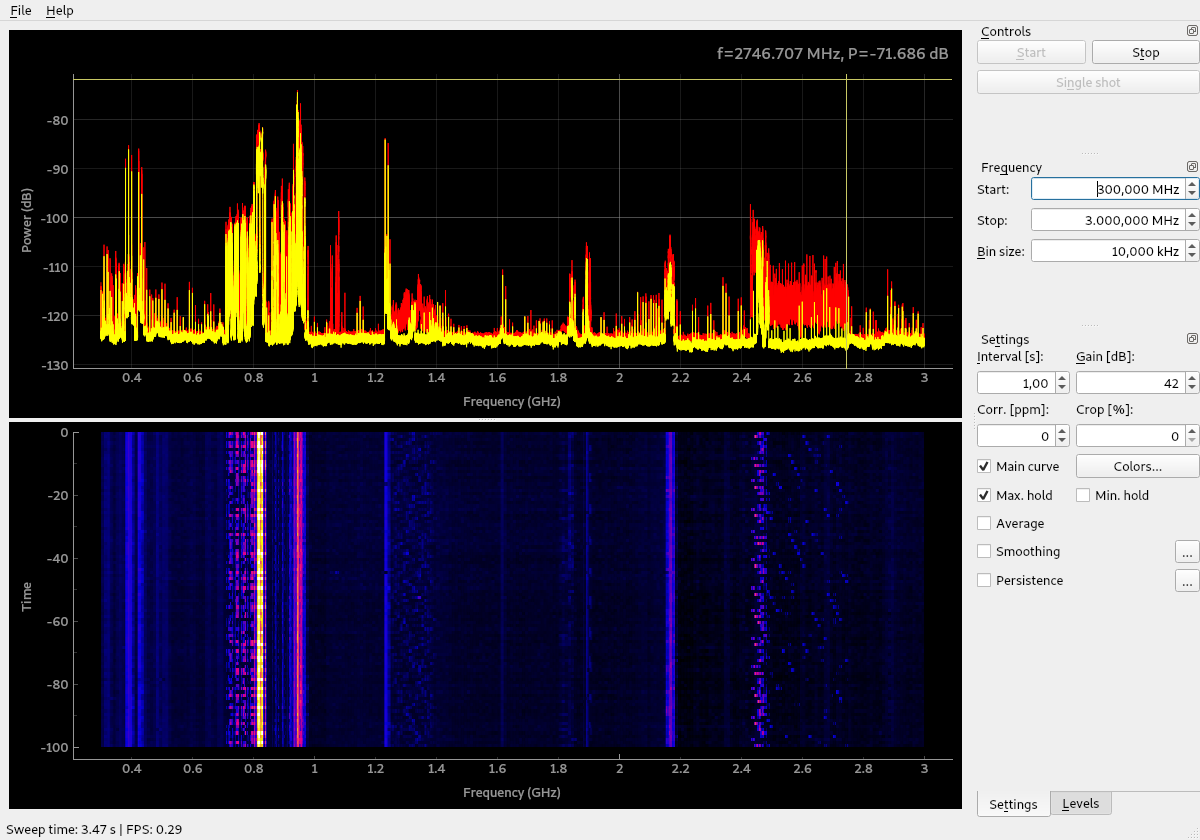
\includegraphics[width=\textwidth]{spektrum.png}
	\caption[Spektralanalyse der Dezimeterwelle]{Spektralanalyse der Dezimeterwelle. Quelle: Eigene Darstellung} 
	\label{spektralanalyse}
\end{figure}


\section{Aufbau/Entwurf}
Zu Beginn der praktischen Arbeit, wird der technische Versuchsaufbau beschrieben. Mit einer Skizze soll der Aufbau der Aufgabe detaillierte dargestellt werden. Wie in der Abbildung \ref{Technischer Aufbau} angezeigt, wird der Computer über den USB-Anschluss mit dem HackRF One verbunden. Darüber bezieht das SDR-Gerät seine notwendige Spannungsversorgung von 5 Volt.\\
Die gegenüberliegende Seite befasst sich mit der Inbetriebnahme der ausgewählten Antenne. Diese hat einen N-Buchsen Anschluss und wird an den HackRF One angeschlossen dieser besitzt jedoch nur einen SMA-Anschluss. Dämpfung wird bei diesem Aufbau nicht berücksichtigt, da das Antennenkabel nur 10 Meter beträgt. Somit können die Geräte miteinander Kommunizieren und die empfangen Daten der Antenne bis hin zum Computer übertragen werden.  
\begin{figure}[H]
	\centering
	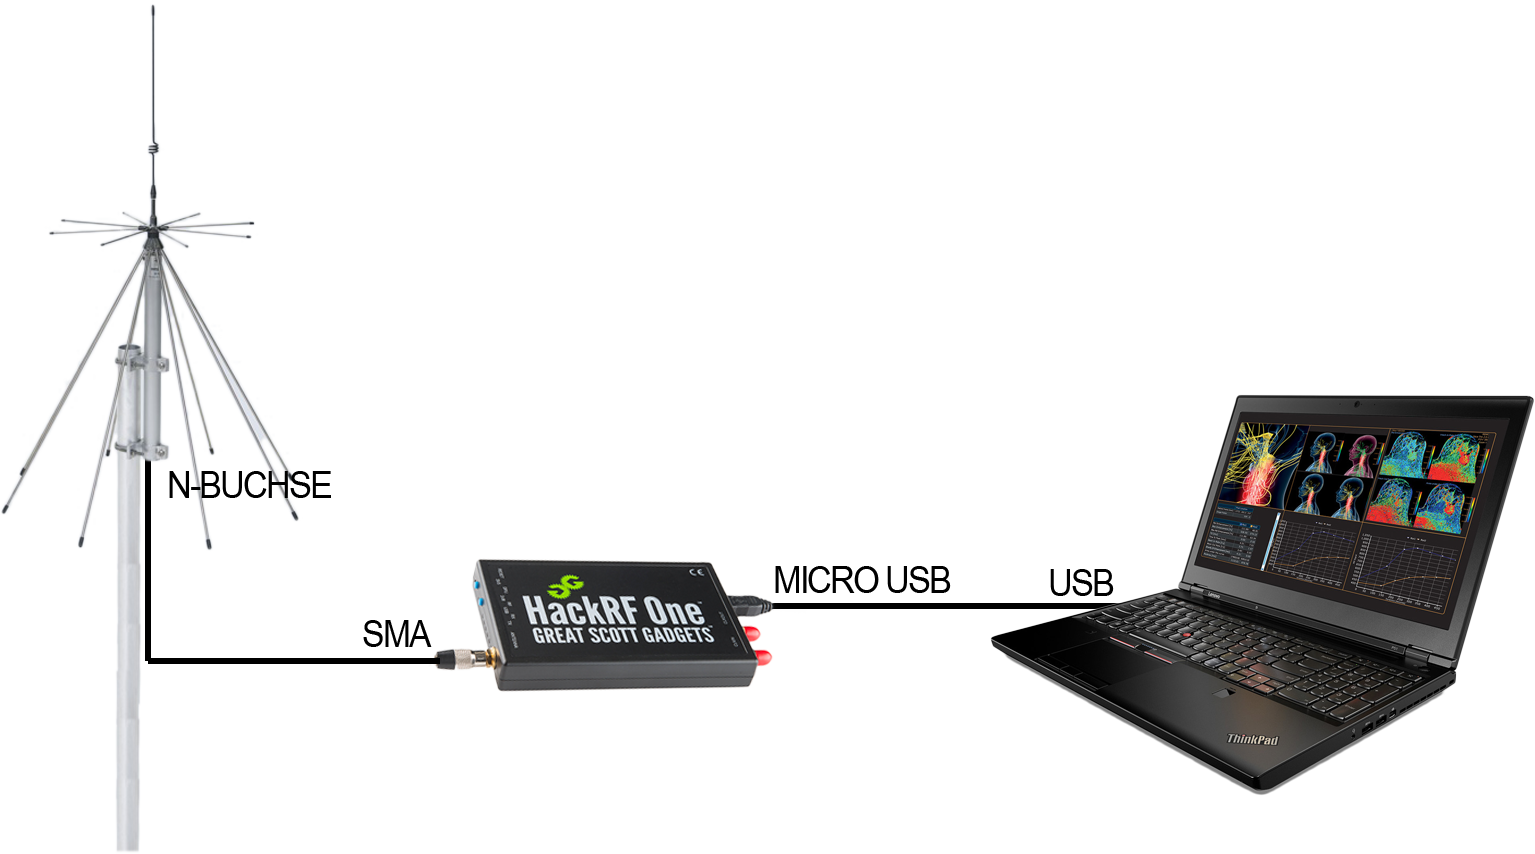
\includegraphics[width=1.0\textwidth]{TechnischerAufbau.png}
	\caption[Technischer Aufbau]{Technischer Aufbau} 
	\label{Technischer Aufbau}
\end{figure}

\section{SDR Sharp}
SDR\# (gesprochen: \enquote{SDR Sharp}) ist eine kostenlose Software von Airspy \cite{airspy:2018}, die ausschließlich für Microsoft Windows erhältlich ist. Mit dieser Anwendung lassen sich u. a. mittels Software Defined Radio Systemen empfangene Signale auslesen und etwa im Frequenzbereich oder in einem Wasserfalldiagramm visualisieren.
So lassen sich einige Modulationsarten relativ schnell und rein visuell identifizieren.
%TODO Bild von SDR# hinzufügen: Am besten ein FM Radiosignal, und erklären woran man die FM Modulation erkennt.


\section{GNU Radio}
GNU Radio \cite{gnuradio} ist ein freies, quelloffenes Entwicklerwerkzeug zur Implementierung von Software Defined Radio mittels Signalverarbeitungsblöcken. Es kann mit externer Funkhardware oder als Simulation ohne zusätzliche Hardware genutzt werden. GNU Radio ist im Hobbybereich weit verbreitet, wird aber auch in der Wissenschaft und im kommerziellen Bereich genutzt. GNU Radio Programme können zusätzlich durch selbst programmierte Ergänzungsblöcke erweitert werden. Die können wahlweise in den Programmiersprachen Python oder C++ geschrieben werden, wobei sich besonders für echtzeitkritische Signalverarbeitungen letzteres anbietet.\\
GNU Radio bietet zusätzlich eine grafische Oberfläche mit \ac{GRC}, die es ermöglicht Blockschaltbilder als Flowgraph darzustellen.

\subsection{Funktionsweise}
GNU Radio verarbeitet den Datenstrom, der vom Empfänger kommt, oder bereitet Daten vor, um diese zu senden. Dabei ist die gesamte Datenverarbeitung in Blöcke eingeteilt, die  beliebig  zusammengestellt  werden können. GNU Radio liefert eine Vielzahl von Filtern, Kanal-Codes, Synchronisationselementen, Equalizern, Demodulatoren, und weitere gängige Werkzeuge der Nachrichten- und Funktechnik. Diese Blöcke stellen die Hardwarekomponenten klassischer Funkhardware dar. Falls nötig können auch selbst Blöcke hinzugefügt werden. Dabei sollte darauf geachtet werden, dass ein Block genau eine Aufgabe erledigt, damit er so vielseitig wie möglich eingesetzt werden kann. GNU Radio bietet die Möglichkeit, diese Blöcke miteinander zu verbinden und regelt dadurch den Datenfluss zwischen verbundenen Blöcken. \\

Für die digitale Verarbeitung von Daten kommen in GNU Radio verschiedene Datentypen zum Einsatz: Der Datenstrom des Empfängers besteht in den meisten Fällen aus komplexen Zahlen, also einem Datentyp, bei dem jedes Datum aus zwei Float-Werten, dem Imaginärteil und dem Realteil, besteht (siehe Abschnitt \ref{iq}). \\
Als Ein- oder Ausgänge eines Blocks können jedoch verschiedene Datentypen zum Einsatz kommen, üblicherweise Short, Byte, Integer und Float. Der Datentyp am Eingang und Ausgang eines Blockes muss dabei nicht gleich sein.\\

Um mit GNU Radio eine SDR-Anwendung zu erstellen, muss man Blöcke, die die einzelnen Funktionseinheiten darstellen, miteinander zu einem Graphen kombinieren. Sollte ein benötigter Block nicht verfügbar sein, kann man diesen mittels einem Tool selbst hinzufügen. Beim Starten des Graphen ruft GNU Radio nun jeden Block nacheinander auf und stellt sicher, dass Daten von einem Block zum Nächsten weitergereicht werden. Ergebnisse  können  durch  Graphical  User  Interface  (GUI)-Blöcke dargestellt werden. Diese nutzen die freien und plattformübergreifenden GUI-Toolkits.


\section{Hardware}

\subsection{Antenne} %TODO: Sollen wir eine von den Antennen, die wir uns anfangs auchgesucht haben mit unserer vergleichen und eine Entscheidungsmatrix aufstellen?  SO dass man sieht, dass wir uns Alternativen angeschaut haben?
Eine Antenne die aus der Aufgabenstellung hervorgeht, muss dementsprechend den Frequenzbereich der Dezimeterwelle abdecken. 
Grundsätzlich gibt es zwei Möglichkeiten ein solches Analysesystem zu betreiben: Mit stationärer oder mobiler Antenne. Letzteres bietet die Möglichkeit das Gerät auch unterwegs nutzen. 
Aus Gründen wie Flexibilität und Mobilität wurde dagegen argumentiert. Eine mobile Antenne, die den Frequenzbereich der Dezimeterwelle abdeckt, würde relativ groß und ziemlich teuer im Vergleich sein. Deshalb kam solch eine Lösungsmöglichkeit nicht in Frage, sondern nur eine stationäre Antenne, da diese preislich 
als auch dem Verwendungszweck dennoch am Nähsten kommt. Die Anforderungen an die Antenne ind :
Größe, Frequenzebereich Datenblatt Die  Sirio SD 3000N erfüllt alle Anforderungen der Aufgabe und ihr Preis liegt bei 90 Euro, was sich optimal in das Preisleistungsverhätlnis integriert.
%TODO: Was sind genau die Vorteile unserer Antenne? -> Aufzählen

\begin{figure}[ht]
	\centering
	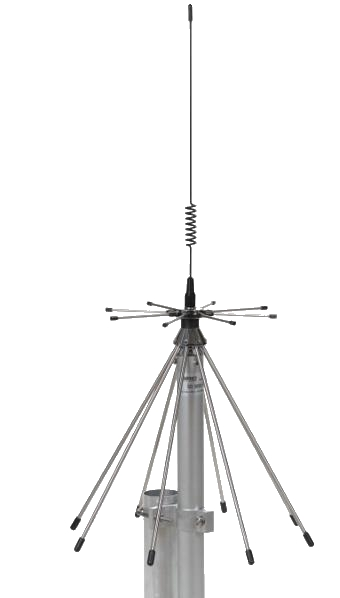
\includegraphics[width=0.4\textwidth]{SirioSD3000N.png} %TODO: Antenne bzw. Bestandteile beschriften? 
	\caption[Sirio SD 3000N stationäre Funkantenne]{Sirio SD 3000N stationäre Funkantenne. Quelle: \cite{Funktechnik:2018}} 
	\label{Sirio SD 3000N Antenne}
\end{figure}

Ganz allgemein kann man Antennen als Koppelelemente zwischen geführten und ungeführten elektromagnetischen Wellen, d. h. als Wandler zwischen Leitungs- und Freiraumwellen, auffassen. Quelle ist immer ein elektrischer oder magnetischer Dipol. Durch eine (Raum-)Transformation im Nahbereich, bei der die Richtungen der Felder (innerhalb der Fortpflanzungsgeschwindigkeit) gedreht werden, entsteht im Fernbereich die gelöste Wellenfront einer elektromagnetischen Welle. 

Elektromagnetische Wellen bestehen aus polarisierten elektrischen und magnetischen Feldern, die sich durch Kopplung wechselseitig erzeugen und im Vakuum ohne Verluste als Transversalwellen räumlich ausbreiten. Bei vorgegebenen Randbedingungen liefern die Maxwellschen Gleichungen eine exakte Beschreibung. In der Praxis berechnet man die Abstrahlung der Energie aber durch Näherungsverfahren. 

%Eine Antenne erzeugt immer sowohl elektrische als auch magnetische Felder. Die Grafik erläutert am Beispiel einer resonanten Dipolantenne, wie aus einem Schwingkreis aus Kondensator und Spule (Start der Animation) durch räumliche Erweiterung (ausklappen der Stäbe, bzw. Erzeugung der Raumtransformation durch 90-Drehung des elektrischen Feldes) eine Antenne entsteht: Die Leiterstäbe werden dabei je um ±90 nach außen gedreht und zwischen den Stäben wirken elektrische Felder (blau gezeichnet); längs der Leiterstäbe wirken magnetische Felder (rot als Kreis gezeichnet). Die Felder breiten sich nicht unendlich schnell, sondern mit Lichtgeschwindigkeit aus und innerhalb dieses sog. „Informationsdurchmessers“ mit v ≤ c sind die Felder über Ursache und Wirkung gekoppelt (Durchmesser der Kugel: λ/2). Wird die Antenne resonant angeregt, bilden sich geschlossene Feldlinien; das sich ändernde elektrische Feld erzeugt zugehörige magnetische Feldlinien, das sich ändernde magnetische Feld erzeugt zugehörige elektrische Feldlinien. Im Nahbereich der Antenne bildet sich ein Blindfeld, d. h., die Ausbreitung der Felder geschieht von der Quelle weg und wieder zurück. Das sich ausbreitende Feld verliert am Randbereich die Kopplung an die Antenne, wenn sich die Richtung der Feldvektoren umkehrt. Die Felder werden durch die Umkehr abgestoßen und können nicht mehr zurück zur Antenne. Eine elektromagnetische Welle wird in den Raum abgestrahlt. Außerhalb des „Informationsdurchmessers“ (Fernfeld) gibt es keine Kopplung an die Antenne mehr, da die Lichtgeschwindigkeit für die Übertragung von Informationen nicht überschritten werden kann. 



Auf Grund analytischen Zwecken haben werden zwei Antennen für die Aufgabe erworben, somit können wir an zwei unterschiedlichen Standorten eine Analyse der Metainformationen betrachten.
Präsentation vom Hochfrequenztechnik aus Mechtronik siehe WhatsApp


\begin{table}[ht]
	\centering
\begin{tabular}{c|c}
	Modell & Sirio SD 3000N\\
	\hline
	Antennentyp & Discone Antenne\\ 
	\hline 
	Bandbreite & 300 MHz - 3 GHz\\ 
	\hline 
	Länge &  72 cm\\ 
	\hline 
	Preis in \euro &  90 \euro \\ 
	\hline 
	Installationsart & Stationär\\ 

\end{tabular} 
	\caption{Produktinformationen der Sirio SD 3000N Antenne}
\end{table}


%TODO: Präsentation vom Hochfrequenztechnik aus Mechtronik siehe WhatsApp

\subsection{SDR-Gerät} %TODO: Struktur in den Text bringen. Absätze, Aufzählungen, etc
Ein Software Defined Radio Gerät, das man experimentell betreiben kann, reicht von mehreren tausend Euro teuren Forschungsgeräte bis zu kostenlosen Geräten, da selbst mittels einem Mikrofoneingang der Soundkarte am Computers, manche Signale empfangen werden können. Die Geräte unterscheiden sich hauptsächlich in Fähigkeiten wie:
\begin{itemize}
	\item Frequenzbereich
	\item maximale Bandbreite
	\item Abtastrate
\end{itemize}

Beim Computer kommen häufig Universal Serial Bus (USB) und Ethernet als Schnittstelle zum  Einsatz.
Da nur Empfängersignale geachtet werden soll, würde ein handelsüblicher DVB-T-Stick eine günstige Option darstellen. Mithilfe des entsprechenden Treibers kann der Stick mit GNU Radio genutzt werden, jedoch deckt sich der Frequenzbereich des Gerätes nicht, mit dem innerhalb der Aufgabenstellung der Dezimeterwelle.\\
Das SDR-Gerät muss in Kombination mit der Funkantenne über den kompletten Frequenzbereich der Dezimeterwelle erstrecken, um die Metainformationen in diesem Bereich zu analysieren. Aus diesem Grund kann ein solchen Gerät für diese Arbeit nicht verwendet werden. Aus der Tabelle können die groben Daten des DVB-T Sticks entnommen werden.\\

\begin{table}[h]
	\centering
	\begin{tabular}{c|c}
		Modellbezeichnung & RTL2832U\\
		\hline
		Hersteller & NooElec\\ 
		\hline 
		Frequenzbereich & 25 MHz - 1750 MHz \\ 
		\hline 
		Preis in \euro & 20 \euro \\ 
		\hline 
		Installationsart & Mobil \\ 
		\hline 
		RX/TX & RX Receiver \\ 
	\end{tabular} 
	\caption{Produktinformationen des HackRF One}
\end{table}

Ein gutes Preis-Leistungsverhältnis bietet das HackRF One Board \cite{greatscott}. Die HackRF One Platine ist ein flexibles Testmodul für die Funkmesstechnik, das wie ein Software Defined Radio (SDR) arbeitet. Sie ist ein Open Source Hardware Transceiver, der hauptsächlich zu eigenen Versuchen und Messungen für SDRs eignet, außerdem ist dieses Gerät für die HF-Technik und messtechnischen Versuchsaufbauten im Amateurfunk vergleichsweise geringen Preises von rund 300 Euro sehr beliebt.\\
Der Hack RF One deckt einen weiten Frequenzbereich von 1 bis 6000 MHz (6 GHz) ab, und erfasst damit sehr viele Frequenzbänder für kommerzielle, experimentelle und Amateurfunk-Anwendungen. Die Hardware bietet eine maximale Abtastrate des Signales von 20MS/s, dadurch werden Messungen und Experimente auch mit breitbandigen Signalen wie DECT, WFM oder WLAN möglich, jedoch nur halbduplex. Der AD-Wandler arbeitet mit 8 Bit Datenbreite und erreicht somit einen theoretischen Dynamikbereich von 48dB. Die digitalisierten I/Q Daten werden auf einem nachgeschalteten CPLD weiterverarbeitet und über den integrierten ARM-Prozessor per USB ausgegeben. Die gesamte Schaltung des HackRF Boards ist sehr stromsparend ausgelegt, sie wird komplett über USB versorgt. Die Platine hat eine Mikro-B USB Buchse. Abschließend lässt sich sagen, dass die oben genannten Gründe für eine Nutzung dieses Gerätes sprechen \cite{wimo:2018}.\\

Eine teure aber auch qualitative Variante bietet das keine Ahnung muss %TODO: Welches Gerät

Abschließend lässt sich das Ergebnis in einer Tabelle visualisieren, darin werden die groben Gesichtspunkte der jeweiligen Komponenten verglichen und auf die Aufgabenstellung untersucht.\\


\begin{figure}[ht]
	\centering
	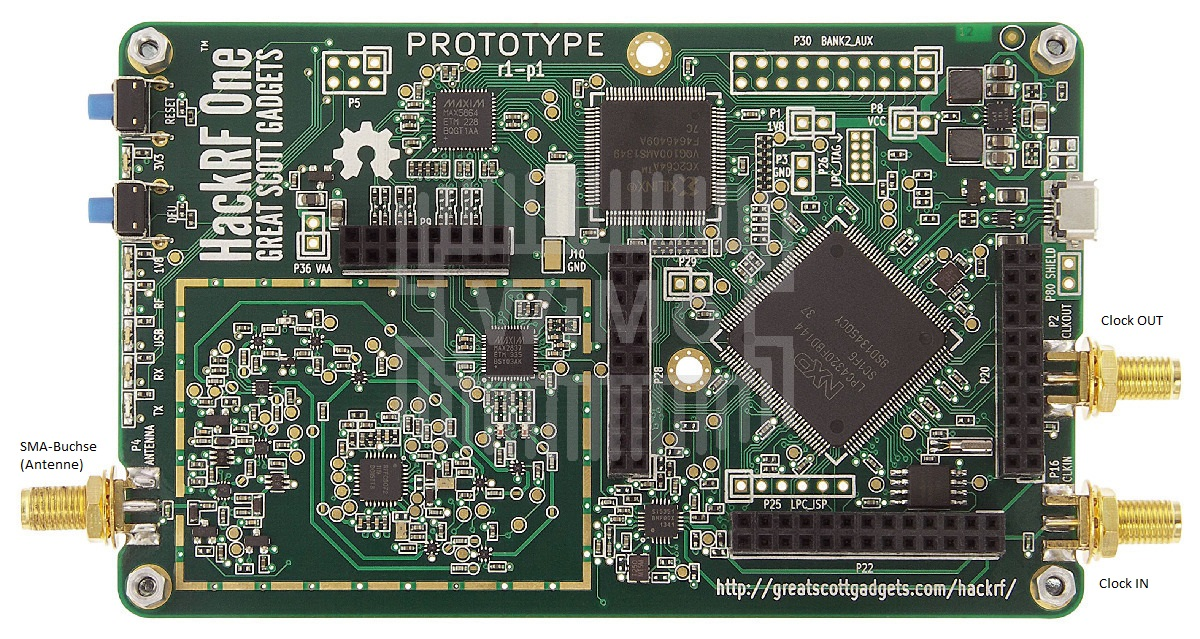
\includegraphics[width=0.75\textwidth]{HackRFOne.png}
	\caption[Hack RF ONE Platine]{Hack RF ONE Platine. Quelle: \cite{HackRFOne:2018}} 
	\label{HackRFOne}
\end{figure}


\begin{table}[ht]
	\centering
	\begin{tabular}{c|c}
		Modellbezeichnung & HackRF One  \\
		\hline
		Hersteller & Great Scott Gadgets\\ 
		\hline 
		Bandbreite & 20 MHz \\ 
		\hline 
		Dynamikumfang & 48 dB \\ %http://www.dolstra.nl/Ham-radio/SDR_Tranceivers/HackRF%20One%20SDR/HackRF%20One%20SDR.htm
		\hline 
		Abtastrate & \( 20 \times 10^{6} \) Hz \\ 
		\hline 
		Preis in \euro &  300 \euro\\ 
		\hline 
		Installationsart & Mobil \\ 
		\hline 
		RX/TX & RX/TX halb-duplex \\ 
	\end{tabular} 
	\caption{Produktinformationen des HackRF One}
\end{table}


\begin{figure}[ht]
	\centering
	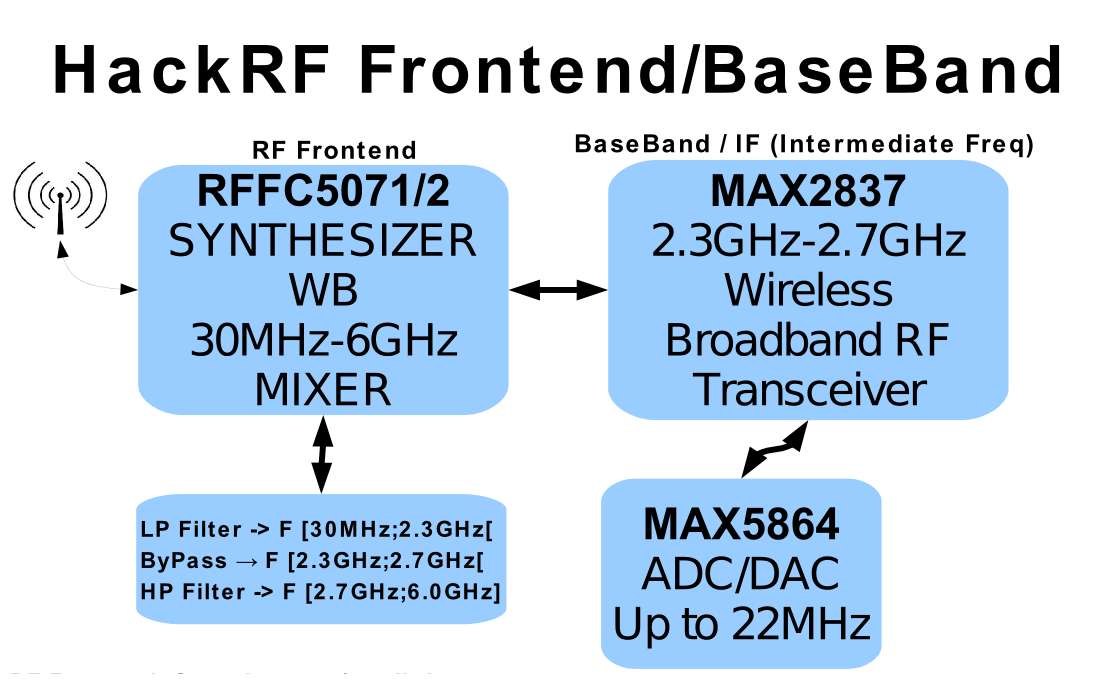
\includegraphics[width=0.7\textwidth]{hackrf-blockdiagram-frontend-baseband.png}
	\caption[Hack RF One Frontend/Baseband]{Hack RF One Frontend/Baseband. Quelle: \cite{hackrf-wiki:2016}} 
	\label{HackRFOne-Blockschaltbild}
\end{figure}
